\chapter{Resultados e discussão}

\begin{justifying}
\section{Diversidade genômica de SARS-CoV-2 em Foz do Iguaçu - Paraná/BR}

No total, excluindo sequências de amostras ambientais, 640 sequências foram utilizadas nas análises. De acordo com a classificação realizada pelo GISAID, foram detectadas 34 variantes em Foz do Iguaçu/PR no período entre 01/01/2020 e 01/01/2023. A quantidade de genomas sequenciados foram 9 (1.5\%), 265 (45.68\%), 197 (33.96\%) e 109 (18.7\%) para a primeira onda (Fev/2020 a Out/2020) , segunda onda (Nov/2020 a Dez/2021), terceira onda (Jan/2022 a Mai/2022) e o segundo semestre de 2022, respectivamente (Figura \ref{fig:fig7}A). 

Essa diversidade genômica contribui para compreender a prevalência das mutações durante as ondas epidemiológicas de SARS-CoV-2. Na cidade da tríplice fronteira, a primeira onda foi marcada pela presença das variantes B.1.1.28 e B.1.1.33. A segunda onda foi marcada pela predominância das variantes P.2 (Zeta), P.1 (Gamma), P.1.7 (Gamma) e sub-linhagens Delta (AY.101, AY.99.2, AY.46.3 e AY.122), respectivamente. A terceira onda  (Jan/2022 a Mai/2022) possuiu uma maior diversidade de variantes em relação às duas primeiras fases, sendo marcada majoritariamente pela circulação de sub-linhagens Ômicron/BA.1.* e BA.2.*. No segundo semestre de 2022, houve uma predominância da variante Ômicron/BA.5.2.1 em relação às demais variantes, assim como, uma diminuição no número de genomas sequenciados.

As variantes Gamma e Zeta surgiram durante a segunda onda, com a variante Gamma emergindo ao final do mês de Novembro/2020, no município de Manaus/AM. Enquanto a variante Zeta foi descrita em Outubro/2020, no município do Rio de Janeiro/RJ. No entanto, estudos anteriores apresentam indícios do surgimento da variante Zeta no estado do Paraná ao final de Agosto/2020, tendo detecções originadas em diferentes localidades da região Sul e Sudeste \cite{Faria:2021, Giovanetti:2022}. Essa constatação é similar com o comportamento epidemiológico observado no município de Foz do Iguaçu, onde a Zeta foi detectada dois meses antes da Gamma (Figura \ref{fig:fig7}A).

Ao final da segunda onda, as variantes Delta foram detectadas majoritariamente. Com exceção da Venezuela e Guianas, países da América do Sul não tiveram uma ressurgência com essas variantes \cite{Graf:2024}. No entanto, sua prevalência no sul brasileiro foi notória em relação às demais linhagens, tendo indícios do surgimento da AY.101 no Estado do Paraná \cite{Arantes:2022}.

\begin{wrapfigure}{c}{\textwidth}
    \centering
    \caption{\justifying Diversidade de linhagens de SARS-CoV-2 em Foz do Iguaçu/PR de Mar/2020 a Dez/2022. (A) Prevalência relativa das linhagens ao longo dos meses, quadro superior apresentando o número de genomas sequenciados, linhas superiores demonstrando o período das ondas de acordo com estudos prévios \cite{Bastos:2021, Giovanetti:2022, Graf:2024, Moura:2022}; (B) perfil alélico de pacientes do HMPGL obtido a partir do estudo experimental, quadro superior apresentando o número de amostras sequenciadas. Mês correspondente a data de detecção/admissão.}
    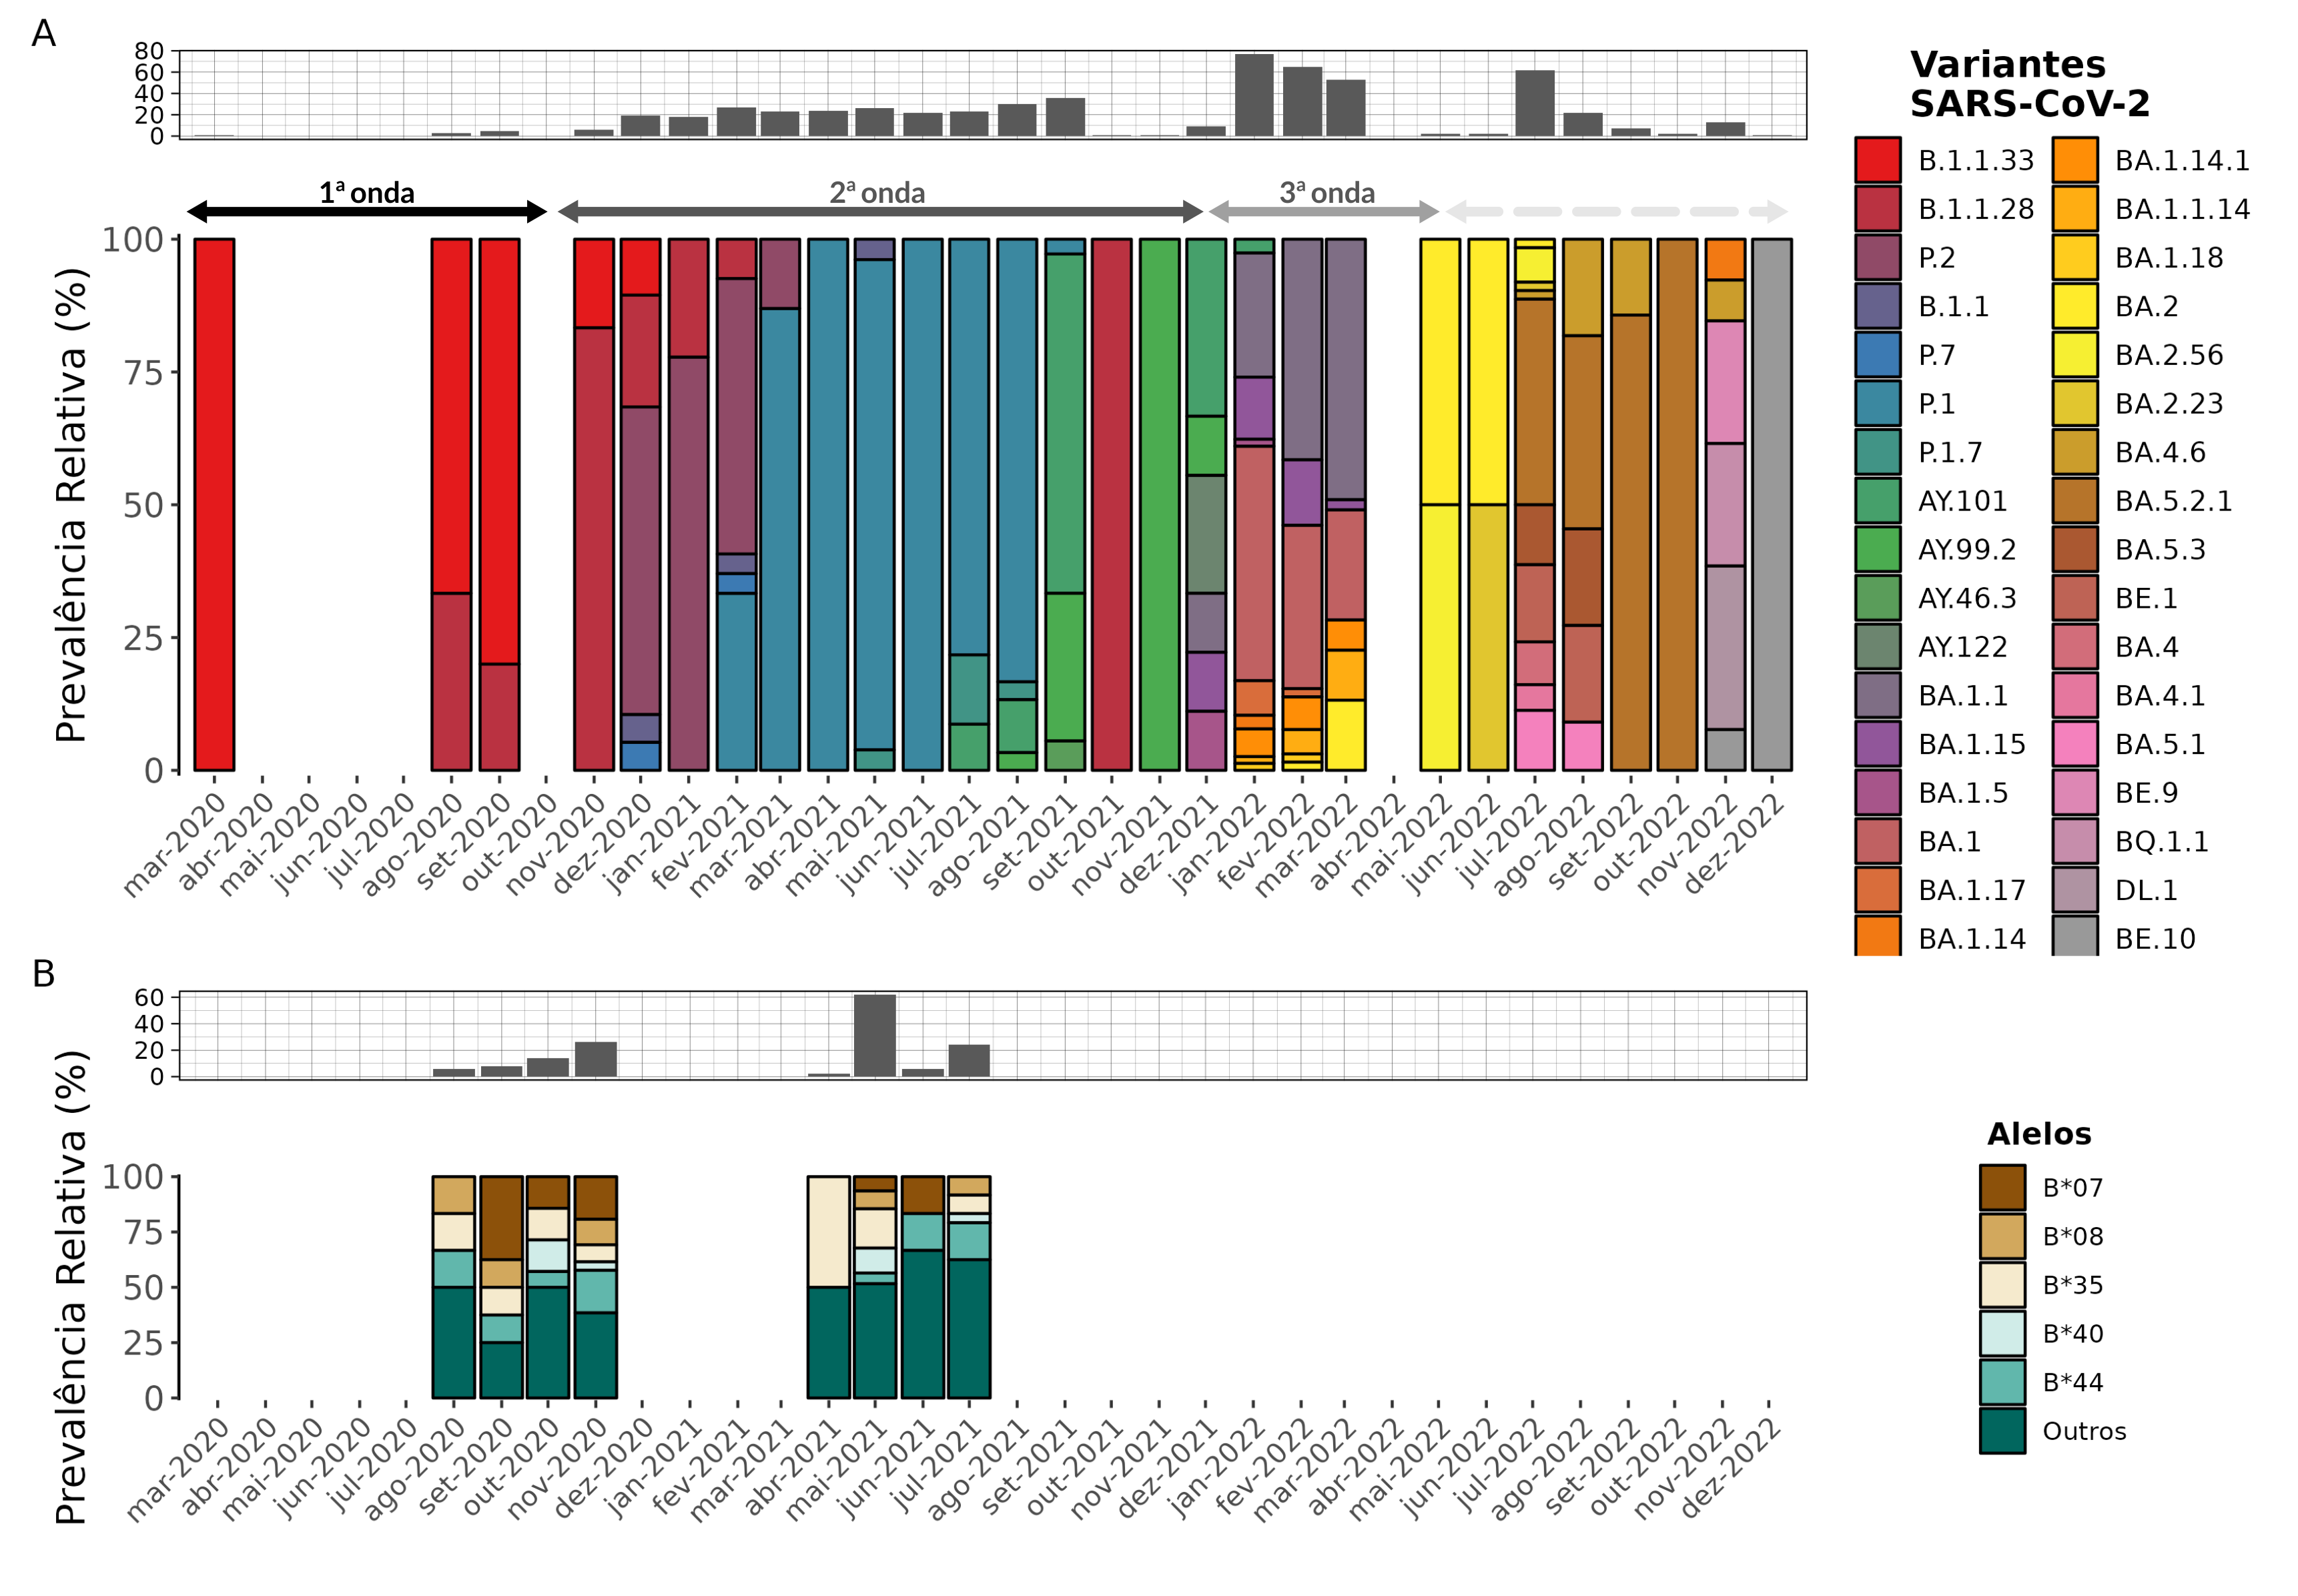
\includegraphics[width=1\textwidth]{Figuras/fig7.png}
    \label{fig:fig7}
    \begin{minipage}{0.8\textwidth} % Adjust width as needed
        \centering
        \footnotesize Fonte: O Autor (2024)
    \end{minipage}
\end{wrapfigure}

\begin{wrapfigure}{c}{0pt}
\end{wrapfigure}

\vspace{10mm}

A composição das variantes das duas primeiras ondas foi comparada de forma indireta com o perfil alélico de pacientes admitidos no HMPGL. O estudo experimental obteve o resultado de 74 amostras de pacientes COVID-19, sendo 27 coletados em 2020 e 47 coletados em 2021. O perfil alélico foi obtido para os genes de HLA-B em uma resolução baixa a nível de grupos alélicos, amostras ou resultados com ambiguidades não foram tratados. Alelos que apresentaram um número total de ocorrências inferior a dez foram agrupados em ``Outros'' (Figura \ref{fig:fig7}B).

O B*07 apresentou diferença significativa entre os anos de coleta (p = 0.02) e óbitos (p = 0.004) em 2020 e 2021, esse último sugerindo uma mudança na ocorrência em pacientes com alta e óbito (Tabela \ref{tab1}). Já o B*41 apresentou diferença entre os desfechos para 2020, mas não atingiu o limiar de significância. Quando ajustado os p-valores para múltiplas comparações, no entanto, os p-valores perdem significância. O grupo alélico B*35 apresentou diferença entre os desfechos de cada ano, mas não foi detectada significância. 

\begin{table}[!h]{14cm}
\caption{Comparações entre as Frequências dos Grupos Alélicos.}\label{tab1}
\scalebox{0.8}{
	\begin{tabular}{ccccccccc}
            \rowcolor[HTML]{999999} 
		\hline
		\textbf{Alelos} 
            & \textbf{\textit{p}} 
            & \textbf{\textit{p.adj}} 
            & \textbf{G1$^1$} 
            & \textbf{G2$^2$}
            & \textbf{G1(n)} 
            & \textbf{G2(n)} 
            & \textbf{Outros 1 (n)} 
            & \textbf{Outros 2 (n)} \\ 
		\hline
		B*41 & 0.052 & 1.0 & Alta20 & Óbito20 & 5 & 0 & 23 & 26 \\
            \rowcolor[HTML]{CCCCCC} 
		B*07 & 0.020 & 0.47 & 2021 & 2020 & 5 & 10 & 89 & 44 \\
            \rowcolor[HTML]{FFFFFF} 
		B*07 & 0.004 & 0.1 & Óbito20 & Óbito21 & 7 & 1 & 19 & 41 \\
		\hline
	\end{tabular}}
        \begin{tablenotes}\footnotesize
         \raggedright
            \item \scriptsize\textit{$^1$}Grupo 1 
            \item \scriptsize\textit{$^2$}Grupo 2
            \par
        \end{tablenotes}
	%\legend{Texto da legenda. (opcional)}
	\source{O Autor (2024)}
\end{table}

Além disso, quando comparadas as frequências relativas com as frequências coletadas do REDOME, o grupo alélico B*07 apresentou uma diferença percentual evidente entre 2020 (18\%), 2021 (5\%) e REDOME (7\%).

\section{Diversidade de mutações \textit{missense} concentra-se em \textit{ORF1ab} e \textit{spike}}

A partir das sequências genômicas, foram gerados 8.222 peptídeos entre \textit{10mers} e \textit{14mers} proveniente das posições de 185 mutações únicas identificadas. As regiões com maior número de mutações \textit{missenses} foi a \textit{ORF1ab} (58), \textit{spike - S} (56) e \textit{Nucleocapsídeo - N} (20), as regiões restantes tiveram menos de 10 mutações. No entanto, a glicoproteína \textit{spike} e as poliproteínas \textit{ORF1ab}  apresentaram maior número de mutações classificadas em \textit{Loss}, 4 e 3, respectivamente. Enquanto a proteína \textit{N} apresentou uma única mutação com forte perda (\textit{Loss}) de afinidade de ligação (Figura \ref{fig:fig8}A).

Além disso, a afinidade de ligação foi mensurada para cada agrupamento. No entanto, como os epítopos não mutados são previstos como não ligantes, essas mutações não foram comparadas com a lista de epítopos validados com alta afinidade de ligação. Ainda é necessário determinar experimentalmente se as mutações do SARS-CoV-2 que aumentam a afinidade dos epítopos ao HLA podem melhorar as respostas das células T e auxiliar no controle do vírus em pacientes com COVID-19.

\begin{wrapfigure}{c}{\textwidth}
    \centering
    \caption{\justifying Número de mutações únicas que levaram ao efeito de (\textit{Weak}) \textit{Gain} ou (\textit{Weak}) \textit{Loss} para (A) cada \textit{ORF}, (B) cada variante e (C) cada alelo. A contagem considera os efeitos para cada alelo predito. Figura B possui as variantes por ordem da primeira detecção na cidade de Foz de Iguaçu de baixo para cima.
}
    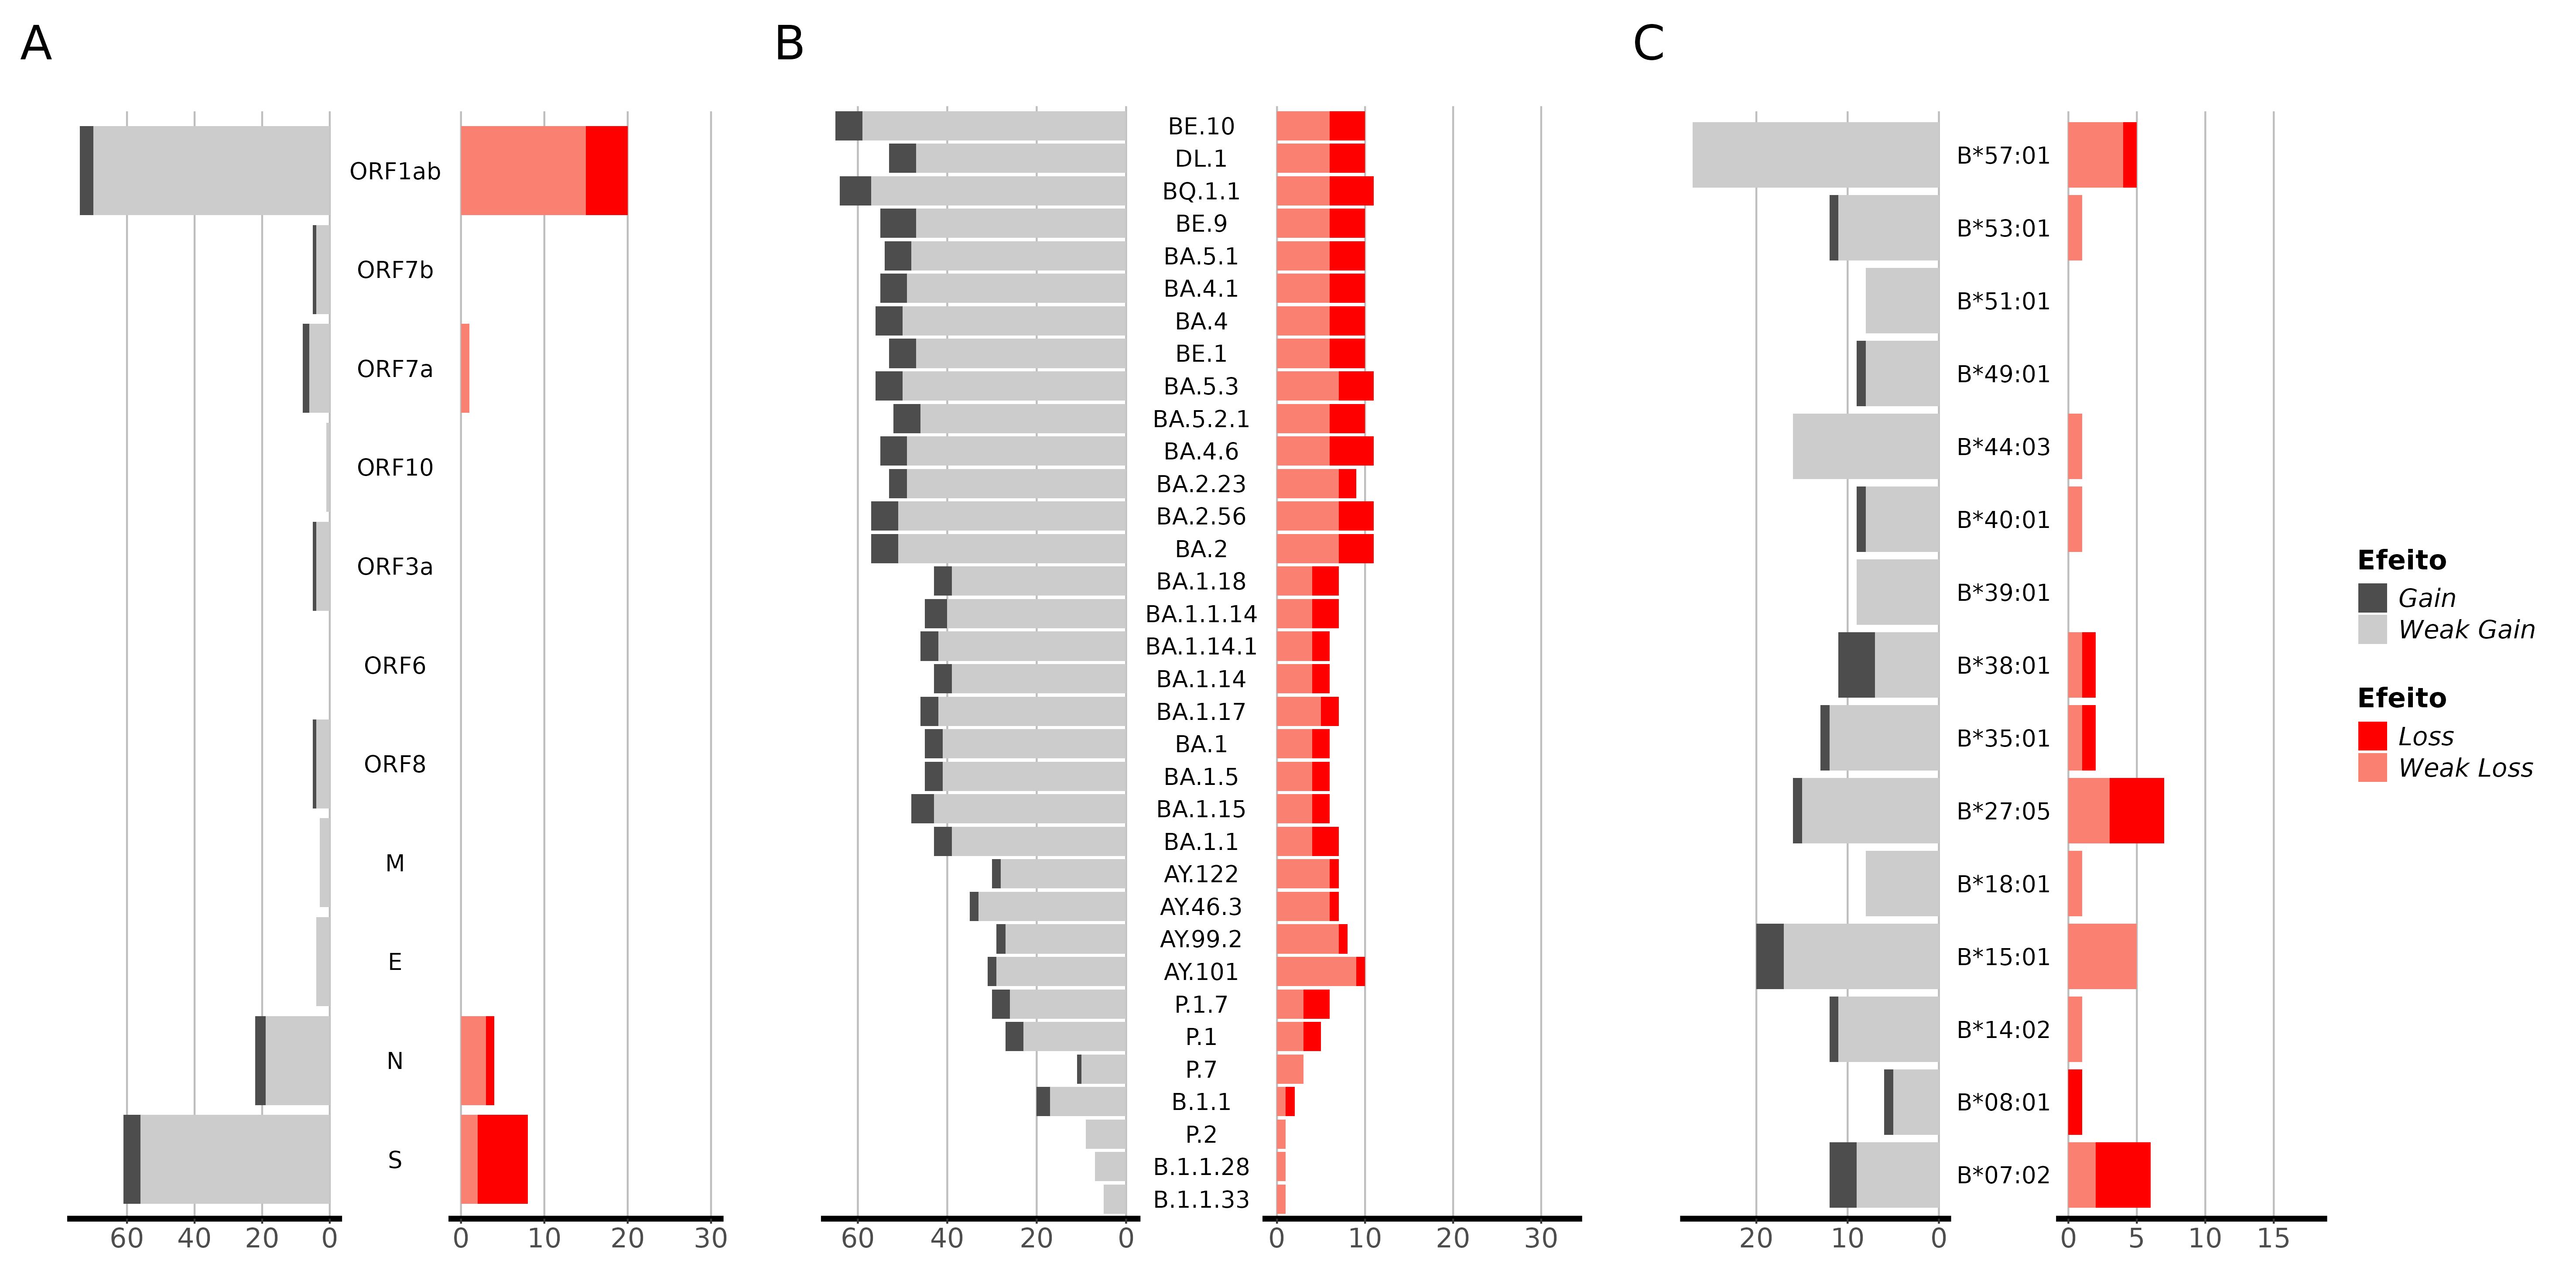
\includegraphics[width=1\textwidth, height=0.5\textwidth]{Figuras/fig8.png}
    \label{fig:fig8}
    \begin{minipage}{0.8\textwidth} % Adjust width as needed
        \centering
        \footnotesize Fonte: O Autor (2024)
    \end{minipage}
\end{wrapfigure}

\begin{wrapfigure}{c}{0pt}
\end{wrapfigure}

\vspace{10mm}

Por outro lado, algumas regiões não possuíram mutações com impacto negativo na predição de afinidade por epítopos. Por exemplo, o envelope apresentou uma única mutação e que não causou qualquer impacto negativo nas análises de afinidade de ligação,  a mutação T9I (posição 9, T$\,\to\,$I) prevaleceu ao longo de 23 variantes. Estudos anteriores sugerem que essa mutação pode estar relacionada à ineficiência do canal de íons transmembrana do vírus, reduzindo a cascata de sinalização intracelular,  resultando em uma diminuição da produção citocinas e diminuição da virulência. Esses fatores podem ter contribuído pelo seu surgimento em Março/2020 e prevalência ao longo das variantes Alfa, Beta, Gamma e Delta em 0,20\%, chegando a 100\% de ocorrência nas variantes Ômicron \cite{Xia:2022}.

Em Foz do Iguaçu, a mutação T9I possivelmente foi introduzida através das variantes Ômicron (BA.*) e tiveram prevalência em variantes posteriores, de BA.1.1 até BE.10. Essa tendência de prevalência pode ser observada na chegada de outras variantes além da Ômicron, as quais contribuíram para o aumento de epítopos mutados que tiveram perda de afinidade de ligação preditas, como no caso das variantes Gamma (P.1 + P.1.7), Zeta (P.2), Delta (AY.101 + AY.99.2 + AY.46.3) (Figura 8B).

Em \textit{ORF1ab}, as mutações com maior prevalência são P323L/P4715L (34), as quais são provenientes da mutação 14408C\textgreater U à nível de nucleotídeo. Esta mutação resulta em uma mutação \textit{missense} P4715L a nível de aminoácidos da poliproteína \textit{ORF1ab} e aparece como mutação P323L na enzima RNA-polimerase RNA-dependente (RdRp). Essa mutação teve uma perda suave na afinidade de ligação em relação ao alelos B*15:01, em conformidade com os relatos da associação dessa mutação com casos severos e elevação na taxa de mortalidade \cite{Toyoshima:2020}.

Outras mutações com frequência significativa em \textit{ORF1ab}, como S135R (13) e P132H/P3395H (23) foram classificados como \textit{Loss}, com as duas últimas mutações levando uma perda de epítopos B*07:02. Esse fato corrobora com análises de bioinformática prévias, as quais sinalizam a perda  de afinidade de epítopos em relação aos alelos HLA-B7 \textit{supertype} \cite{Hamelin:2022}. Na Figura 8C, é possível observar uma tendência dos alelos B*07:02 e B*27:02, principais representantes de HLA-B7 e HLA-B27, na perda de afinidade de ligação a partir de epítopos mutados, contendo o maior número de mutações classificadas como \textit{Loss}, respectivamente.

Em relação à glicoproteína \textit{spike}, a mutação D614G apresentou maior frequência em relação a todas as mutações detectadas na cidade de Foz do Iguaçu, ao total foram 34 variantes portadoras desta mutação (Figura \ref{fig:fig9}A). A D614G não afetou a afinidade de ligação a partir das predições realizadas para os alelos de HLA-B, apesar da sua ocorrência estar ligada ao aumento da taxa de mortalidade, aumento do sinal de detecção de RT-qPCR devido a carga viral e predições relacionadas aos alelos HLA-A \cite{Hamelin:2022, Korber:2020, Toyoshima:2020}. Por outro lado, epítopos com mutações P681H (24), P681R (4), R346K (3) e R346T (2) apresentaram uma perda significativa na afinidade de ligação aos alelos  B*27:05 e B*07:02 para as posições 681 e 346, respectivamente. Enquanto as mutações T95I (10) e V213G (14) foram classificadas como \textit{Weak Loss} em relação à  B*57:01 e B*38:01, respectivamente.  


\begin{wrapfigure}{c}{\textwidth}
    \centering
    \caption{\justifying Distribuição da posição dos epítopos e suas variantes mutadas dos antígenos de SARS-CoV-2 que circularam em Foz do Iguaçu/PR. (A) Posição das mutações ao longo do genoma de SARS-CoV-2, mutações que ocorreram em mais de 20 variantes estão destacadas em amarelo, mutações que foram classificadas como \textit{Gain}, \textit{Loss} e \textit{Weak Loss} estão destacadas em cinza escuro, vermelho e salmão, respectivamente; (B) estrutura de um monômero da \textit{spike} ligado à ACE2. As posições das mutações e região do FCS (680-690) estão destacadas em esferas vermelha e verde, respectivamente. 
}
    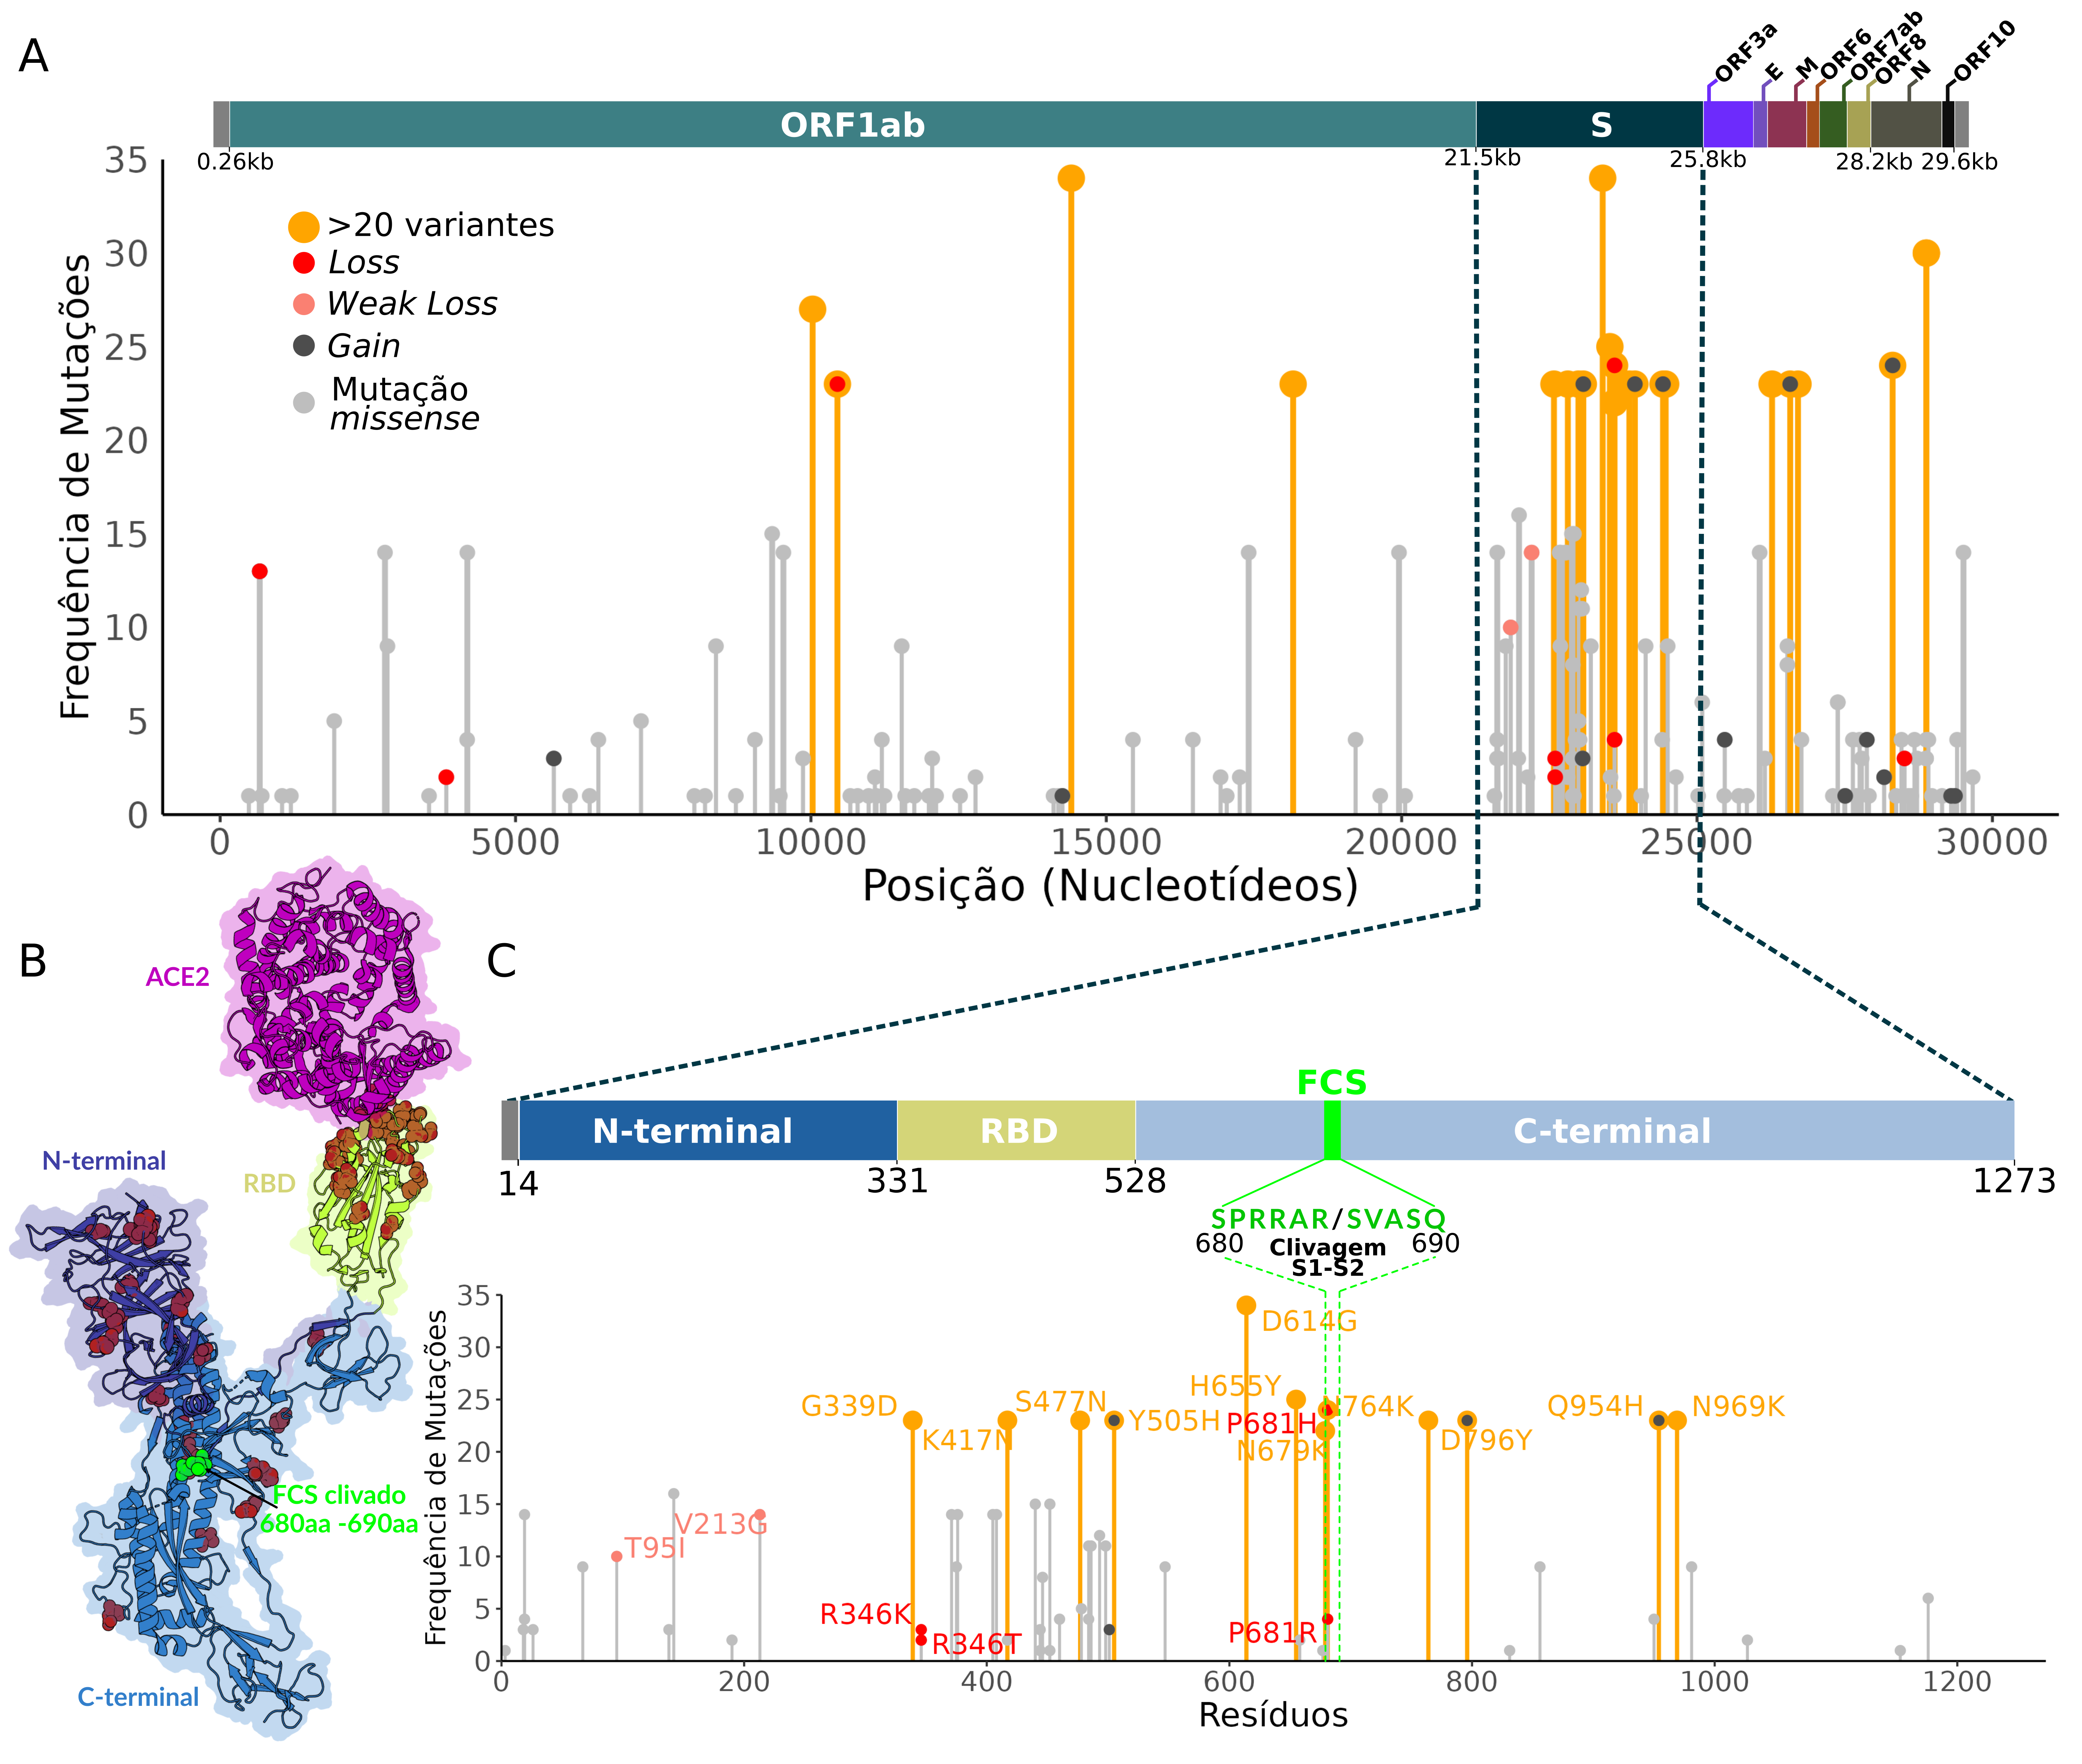
\includegraphics[width=1\textwidth, height=0.8\textwidth]{Figuras/fig9.png}
    \label{fig:fig9}
    \begin{minipage}{0.8\textwidth} % Adjust width as needed
        \centering
        \footnotesize Fonte: O Autor (2024)
    \end{minipage}
\end{wrapfigure}

\begin{wrapfigure}{c}{0pt}
\end{wrapfigure}

\vspace{10mm}


A mutação P681R é exclusivamente carregada por variantes Delta, já a mutação P681H surge a partir de variantes Ômicron em conjunto com mutação N679K (Figura \ref{fig:fig9}C). Essas mutações ocorrem em uma posição adjacente ao ao Sítio de Clivagem da Furina (\textit{FCS}, sigla em inglês) e aumentam o número de aminoácidos básicos, característica crucial para o reconhecimento pela furina \cite{Harvey:2021}.  Além da perda da prolina que afetam a apresentação de epítopos associados à HLA-B7 supertype, mutações na posição 681 também apresentaram resistência à beta interferon (IFN-$\beta$) e conferindo uma evasão em relação ao sistema imune adaptativo e inato \cite{Hamelin:2022, Lista:2022}. 

As mutações na posição R346 surgiram de forma tardia, R346K e R346T foram prevalentes em variantes BA.1.* e BA.4.6/BQ.1.1, respectivamente. Resultados experimentais sugerem que essas mutações podem conferir uma resistência à neutralização por anticorpos previamente identificados por atuarem em antígenos de SARS-CoV-2  \cite{Cao:2022}. A mutação V213G surge de maneira tardia a partir de BA.2.* e  a mutação T95I a partir da variante Delta AY.101 e prevalece ao longo das sub-linhagens Ômicron BA.1.*. 

A glicoproteína spike é essencial para a interação com a enzima de conversão de angiotensina 2 (\textit{ACE2}, sigla em inglês), expresso nas células hospedeiras, e é importante para a transmissão viral, sendo uma região crítica para prevalência de mutações \textit{missense} \cite{Harvey:2021, Piccoli:2020, Toyoshima:2020}. Na Figura \ref{fig:fig9}B e \ref{fig:fig9}C, é possível observar que o domínio de ligação de receptor (\textit{Receptor Binding Domain - RBD}) acumula o maior número de mutações em relação ao C-terminal e N-terminal, região de maior contato com receptores \textit{ACE2}. 

De acordo com \citeonline{Piccoli:2020},  o RBD de SARS-CoV-2 é imunodominante em relação a quantidade total de anticorpos monoclonais elicitados, é alvo de 90\% da atividade neutralizante presente no soro ou plasma de indivíduos infectados e apresenta dois sítios principais na neutralização da fusão do vírus à células hospedeiras pela ligação ao \textit{ACE2}. Além da região \textit{RBD}, as variantes Ômicron possuíram mutações conservadas (H655Y, N679K e P681H) adjacente ao \textit{FCS}, as quais potencializaram a clivagem da proteína \textit{spike} e a fusão com a célula hospedeira \cite{Viana:2022}.  

No entanto, ao contrário das variantes Alpha (P681H) e Delta (P681R), as mutações em \textit{RBD} e \textit{FCS} não foram determinantes para prevalência e alta transmissibilidade das variantes Ômicron. As mudanças genotípicas nas novas variantes do vírus demonstraram alterar o fenótipo viral, modulando as respostas imunes inatas e a evasão da resposta imune adaptativa, além de modificar a funcionalidade da proteína \textit{spike}, afetando a transmissão e a patogênese.  \cite{Harvey:2021, Willett:2022}. Segundo resultados apresentados por \citeonline{Willett:2022}, variantes Ômicron BA.1 e BA.2 mudaram a preferência de via de entrada à célula hospedeira, utilizando um mecanismo de fusão endossômica independente de TMPRSS2, principal protease transmembrana envolvida na fusão do envelope viral. 

Em Foz do Iguaçu, além da D614G, P681* e H655Y que prevalecem na \textit{spike} de diferentes variantes, as mutações mais abundantes ocorreram ao longo da circulação de sub-linhagens Ômicron, evidenciando a diversidade de mutações dessas linhagens que geraram uma série de mecanismos fenotípicos adaptados para sua prevalência ao longo do tempo.  Apesar da mutação D614G surgir amplamente nas variantes da primeira onda, a segunda mutação mais frequente H655Y é compartilhada exclusivamente entre as variantes Gamma P.1 e Ômicron BA.1.1 \cite{Ou:2022}.

\section{Epítopos de B*07:02 apresentam  maior perda na afinidade de ligação com mutações \textit{missense}}

A partir do \textit{pipeline} desenvolvido, foram detectadas 23 epítopos mutados que apresentaram impacto negativo nos valores de afinidade de ligação preditos em relação aos alelos escolhidos de HLA-B. De acordo com a Figura 10A, as variantes apresentaram um acúmulo de mutações classificadas em Weak Loss/Loss ao longo do tempo.  O surgimento de mutações com perdas leves preditas teve maior concentração em ORF1ab (Figura \ref{fig:fig10}A e \ref{fig:fig10}B) e quando ocorreram efeitos negativos, mutações na proteína \textit{spike} geraram um alto impacto na afinidade de ligação predita.

\begin{wrapfigure}{c}{\textwidth}
    \centering
    \caption{\justifying Valores de \textit{Log}$_{2}$(\textit{Fold Change}) para cada mutação classificada em (\textit{Weak}) \textit{Loss}. Mutações classificadas por (A) variantes e (B) por genes. Variantes estão ordenadas de baixo para cima a partir da primeira data de detecção em Foz do Iguaçu. Mutações que geraram Loss estão identificadas com alelo:mutação:\textit{k-mer}  e indicação na lateral esquerda da onda epidemiológica que ocorreu a primeira detecção em (B)}
    \includegraphics[width=1\textwidth, height=0.8\textwidth]{Figuras/fig10.png}
    \label{fig:fig10}
    \begin{minipage}{0.8\textwidth} % Adjust width as needed
        \centering
        \footnotesize Fonte: O Autor (2024)
    \end{minipage}
\end{wrapfigure}

\begin{wrapfigure}{c}{0pt}
\end{wrapfigure}

\vspace{10mm}

Em relação ao perfil de mutações  \textit{Weak Loss}/\textit{Loss} de cada variante, é possível visualizar que foi diferente em cada período marcado pelas ondas epidemiológicas. Como apresentado na Figura \ref{fig:fig9}A, variantes Gamma, Zeta e Delta marcam essa mudança, seguida pelas variantes Ômicron. Curiosamente, as mutações nas primeiras variantes detectadas e com menor magnitude de \textit{fold change} concentram-se em grande parte na \textit{ORF1ab}. Essa região codifica proteínas não estruturais envolvidas na replicação viral e podem tolerar mais mutações, pois estão envolvidas em processos que podem ser menos impactados por mutações pontuais.

Os epítopos mutados classificados com perda apresentaram  1.1-\textit{fold} à 120-\textit{fold} de diminuição nos valores preditos em relação à sequências de referência.  Enquanto isso, os epítopos que apresentaram maior amplitude (\textit{Log2(Fold Change)} $\geq$ 5), entre 34-\textit{fold} à 120-\textit{fold}), possuem prevalência a partir das variantes Gamma (P.1.7) e permanecem ao longo das variantes Ômicron.  As perdas são detectadas quando comparadas a epítopos de referência B*07:02, seguido dos epítopos de B*27:05 (Figura \ref{fig:fig10}B). O momento de surgimento das mutações que atingem epítopos B*07:02 difere ao período de maior número de pacientes internados que carregam o grupo alélico B*07 ao final da primeira onda, segundo os dados experimentais.

A mutação Prolina (P)$\,\to\,$X e Arginina (R)$\,\to\,$X afetam, majoritariamente, os valores preditos para  epítopos B*07:02 e B*27:05, respectivamente. Especialmente, quando localizado na posição âncora do epítopo, nesse caso, P2.  Conforme visualizado na (Tabela \ref{tab2}),   esse tipo de mutação está diretamente relacionada com o aumento da magnitude de \textit{fold change}. Dados similares foram apresentados em estudos anteriores, onde coletaram dados genômicos globais de SARS-CoV-2 e verificaram o impacto negativo nesse tipo de mutação na apresentação alélica de epítopos associados ao HLA-B7 \textit{supertype}, mas um impacto positivo foi apontado para HLA-B27 \textit{supertype}  \cite{Hamelin:2022}. 

% Please add the following required packages to your document preamble:
% \usepackage[table,xcdraw]{xcolor}
% Beamer presentation requires \usepackage{colortbl} instead of \usepackage[table,xcdraw]{xcolor}
\begin{table}[!h]{15.5cm}
\caption{Mutações \textit{Loss} epítopos associados ao alelo B*07:02 e B*27:05}\label{tab2}
\scalebox{0.7}{
\begin{tabular}{cccccccc}
\hline
\rowcolor[HTML]{999999} 
\textbf{Epítopo (Ref/mut)} &
  \textbf{K-mers} &
  \textbf{Gene} &
  \textbf{Alelo} &
  \textbf{Mutação} &
  \textit{\textbf{Log$_2$(FC)}} &
  \textit{\textbf{FC$^1$}} &
  \textbf{Núm. de variantes} \\
  \hline
R\textbf{P/H}NFTIKGSFL   & 11 & ORF1ab & B*07:02 & P132H/P3395H & 6.9  & 120.03 & 23 \\
\rowcolor[HTML]{CCCCCC} 
R\textbf{P/H}NFTIKGSF    & 10 & ORF1ab & B*07:02 & P132H/P3395H & 6.7  & 104.34 & 23 \\
S\textbf{P/R}RRARSVASQSI & 13 & S      & B*07:02 & P681R        & 5.79 & 55.57  & 4  \\
\rowcolor[HTML]{CCCCCC} 
AT\textbf{R/T}FASVYAW    & 10 & S      & B*27:05 & R346T        & 5.75 & 53.98  & 2  \\
T\textbf{R/T}FASVYAWNR   & 11 & S      & B*27:05 & R346T        & 5.43 & 43.23  & 2  \\
\rowcolor[HTML]{CCCCCC} 
S\textbf{P/H}RRARSVASQSI & 13 & S      & B*07:02 & P681H        & 5.41 & 42.72  & 24 \\
AT\textbf{R/K}FASVYAW    & 10 & S      & B*27:05 & R346K        & 3.79 & 13.85  & 3  \\
\rowcolor[HTML]{CCCCCC} 
T\textbf{R/K}FASVYAWNR   & 11 & S      & B*27:05 & R346K        & 3.62 & 12.36  & 3  \\
IPARARV\textbf{E/D}CF    & 10 & ORF1ab & B*07:02 & E341D        & 1.37 & 2.58   & 2  \\
\rowcolor[HTML]{CCCCCC} 
GPQNQRNA\textbf{P/L}RITF & 13 & N      & B*07:02 & P13L         & 1.34 & 2.54   & 24 \\
\rowcolor[HTML]{FFFFFF} 
QNQRNA\textbf{P/L}RITF   & 11 & N      & B*27:05 & P13L         & 0.56 & 1.47   & 24 \\
\rowcolor[HTML]{CCCCCC} 
ARL\textbf{R/C}AKHYVY    & 10 & ORF1ab & B*27:05 & R5716C/R392C & 0.51 & 1.43   & 14 \\
\rowcolor[HTML]{FFFFFF} 
ARL\textbf{R/C}AKHYVY    & 10 & ORF1ab & B*27:05 & R5716C/R392C & 0.51 & 1.43   & 14 \\
\rowcolor[HTML]{CCCCCC} 
RRIRGGDGK\textbf{M/I}K   & 11 & N      & B*27:05 & M101I        & 0.32 & 1.25   & 1 \\
\hline
\end{tabular}}
    \begin{tablenotes}\footnotesize
    \raggedright
        \item \scriptsize\textit{$^1$}\textit{Fold Change}
        \par
    \end{tablenotes}
\source{O Autor (2024)}
\end{table}


Em relação a alta prevalência, os epítopos gerados pelas mutações P323L/P4715L (VLFSTVFPP/LTSF) do \textit{RdRp} (\textit{ORF1ab}) estão presentes no genoma de todas as variantes que circularam em Foz do Iguaçu, sendo a mutação mais prevalente fora da região da proteína \textit{spike} e foi classificada como \textit{Weak Loss} em relação aos epítopos B*15:01. Estudos anteriores apontam que a mutação P323L favorece a estabilidade estrutural da \textit{nsp12} e afeta diretamente a sua função por meio da interação da sua posição com co-fatores \textit{nsp7} e \textit{nsp8} - aumentando a taxa de mutação no processo de tradução \cite{Kim:2023, kirchdoerfer:2019}. Além disso, observa-se uma coevolução significativa entre as mutações D614G e P323L, na qual a presença isolada de G614 ou L323 não ganhou relevância epidemiológica. Em contrapartida, a combinação dessas duas mutações resultou em uma variante viral G/L que quase completamente substituiu a variante original D/P \cite{Ilmjarv:2021}.

Por fim, é possível identificar que epítopos associados ao B*07:02 e B*27:05 obtiveram uma maior magnitude de \textit{fold change} a partir do surgimento de mutações (Figura \ref{fig:fig11}). Apesar de dados \textit{in silico} não confirmarem o papel das mutações no escape imunogênico de epítopos associados à B*27:05 como apontado para B*07:02, estudos experimentais com células CD8+ corroboram com o impacto negativo de mutações em epítopos associados a ambos alelos \cite{Wellington:2023}. 

\begin{wrapfigure}{c}{\textwidth}
    \centering
    \caption{\justifying Comparação entre a predição da afinidade de ligação em escala logarítmica (eixo y) de epítopos com mutações e referência (eixo x) para cada alelo. \textit{Total Loss} são todas as classificações \textit{Weak Loss} e \textit{Loss} e p-valores se encontram na parte superior de cada quadro.}
    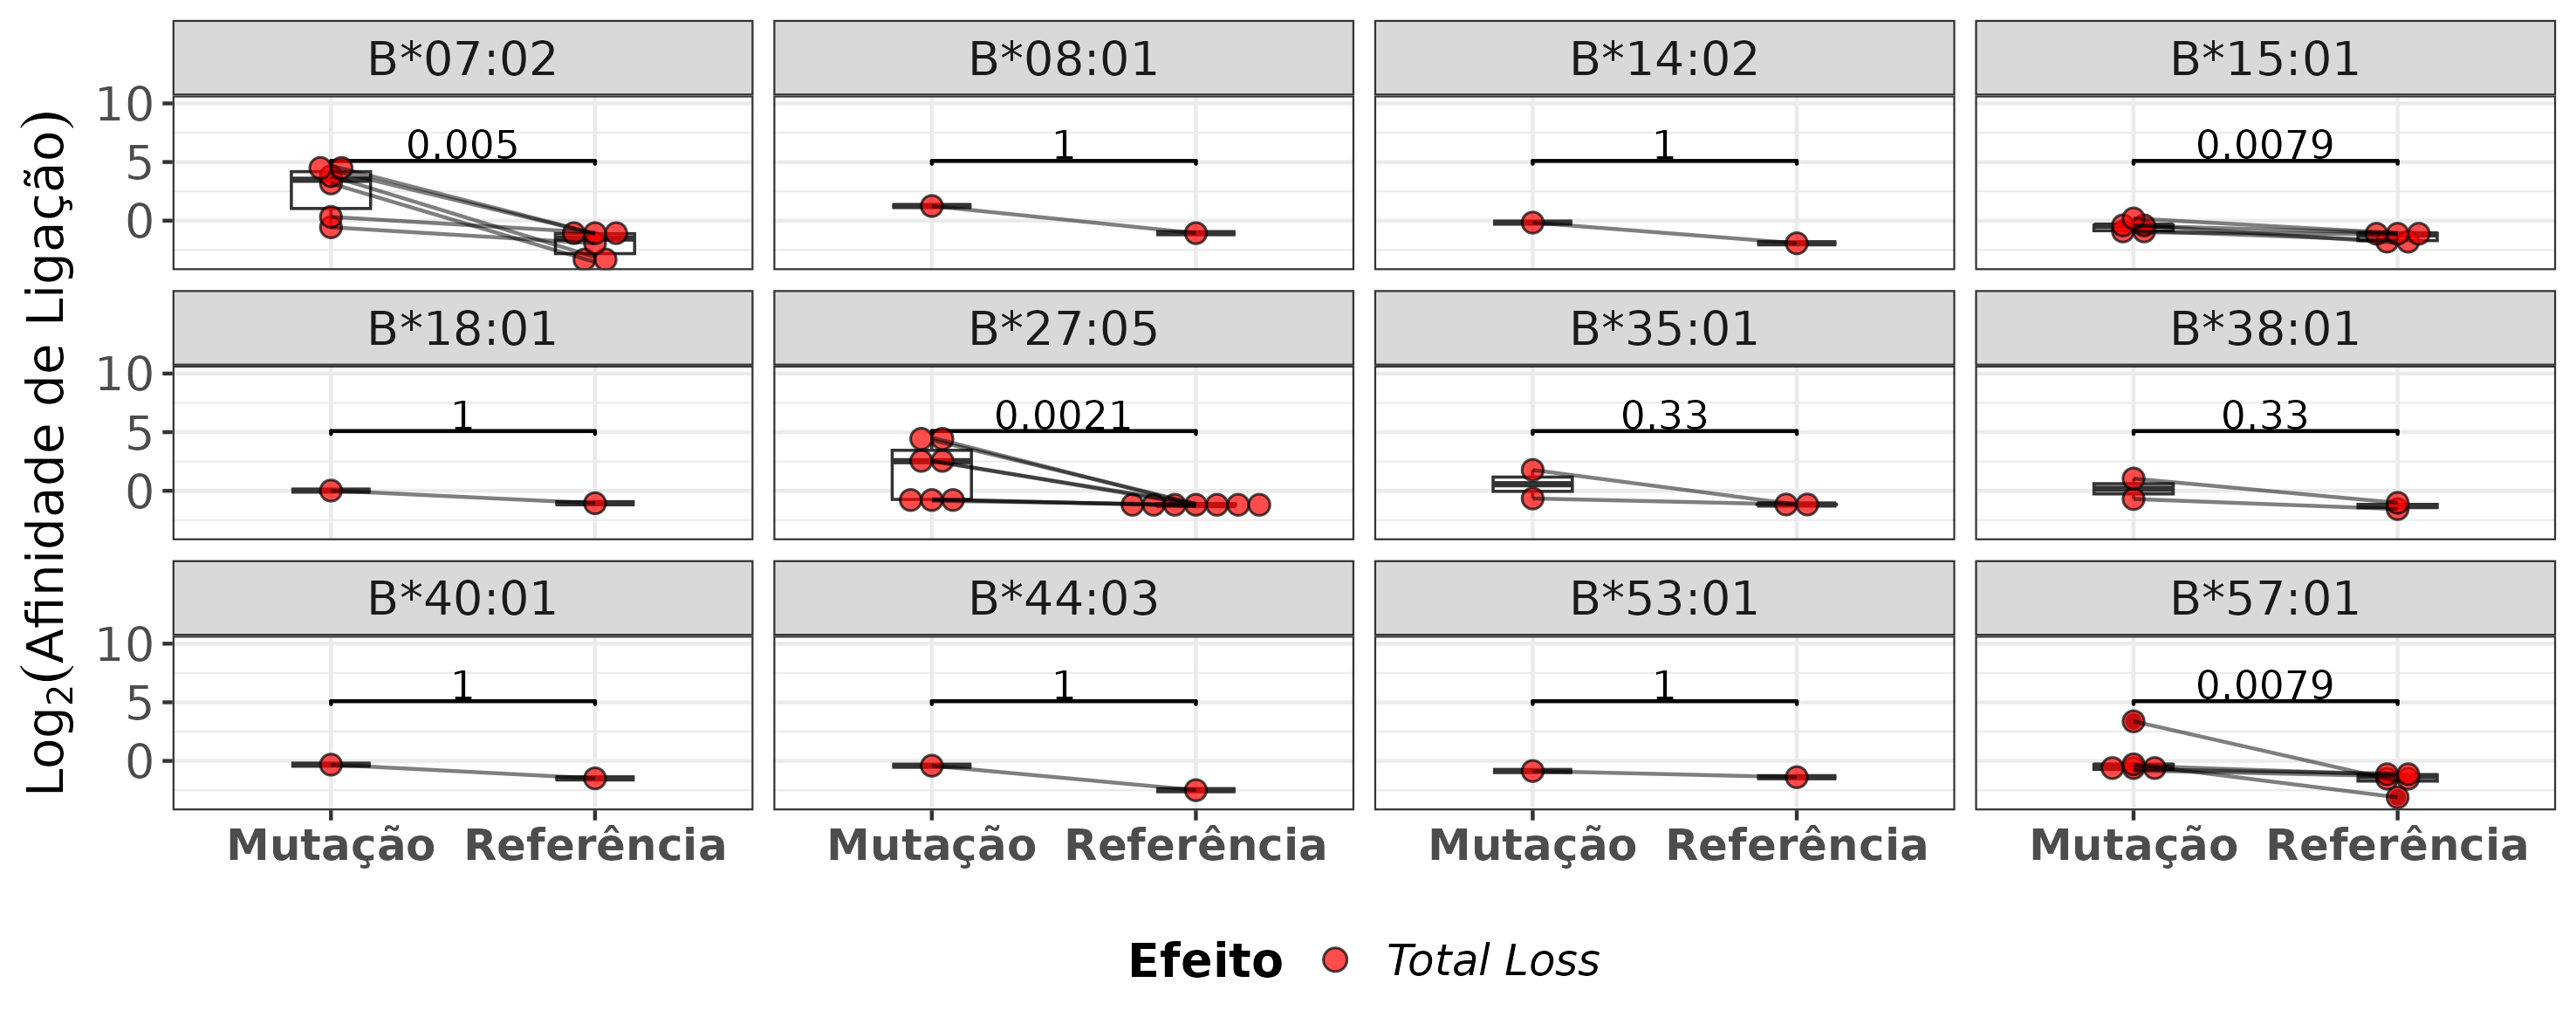
\includegraphics[width=0.8\textwidth, height=0.4\textwidth]{Figuras/fig11.png}
    \label{fig:fig11}
    \begin{minipage}{0.8\textwidth} % Adjust width as needed
        \centering
        \footnotesize Fonte: O Autor (2024)
    \end{minipage}
\end{wrapfigure}

\begin{wrapfigure}{c}{0pt}
\end{wrapfigure}

\vspace{2cm}

\section{Implicações e limitações do estudo na região de fronteira}

Ao final de 2020, o surgimento de Variantes de Interesse (\textit{VOI}, sigla em inglês) e Variantes de Preocupação (\textit{VOC}, sigla em inglês) gerou a ocorrência de novas ondas epidemiológicas, apresentando perfil de transmissibilidade e patogênese diferente quando comparada às variantes iniciais. A origem de mutações nas novas variantes com alta prevalência instigaram buscar compreender seus impactos no escape do sistema imune humano e considerá-las fatores importantes durante o desenvolvimento de vacinas ou guiando na decisão de políticas públicas no combate ao vírus.	

O município  de Foz do Iguaçu está localizado em uma área de tríplice fronteira com potencial exportação e importação de novas variantes, ou seja, servindo como área estratégica na contenção de ondas epidemiológicas causadas por novas variantes. Situada na fronteira entre Brasil, Paraguai e Argentina, a cidade possui fronteiras terrestres entre os três países e com uma atividade socioeconômica baseada no turismo e no trânsito comercial aduaneiro. Durante a pandemia de COVID-19, a cidade contou com a flexibilização de medidas de segurança sanitária, especialmente, a permanência do funcionamento de hotéis, aeroporto, rodoviária e a reabertura das fronteiras \cite{Rivas:2020}. 

Os laboratórios de detecção molecular de SARS-CoV-2 foram empregados para realizar um monitoramento de casos no município, localizados no Hospital Municipal Padre Germano Lauck (HMPGL) e Hospital Ministro Costa Cavalcanti (HMCC). Os esforços na detecção de casos de COVID-19 também se estenderam no rastreamento de variantes, realizando coleta e sequenciamento de genomas de SARS-CoV-2 em diferentes períodos epidemiológicos. No início da pandemia, adicionalmente, a Universidade Federal da Integração Latino-Americana (UNILA) apresentou um amplo estudo buscando compreender a imunidade humoral e celular de casos assintomáticos no município \cite{Viana:2021}. 

Apesar desses dados serem armazenados em bancos públicos, como o GISAID e DATASUS,  ou publicados em artigos científicos em conjunto com dados de demais regiões do Brasil, não houve uma abordagem que examinasse  a circulação de variantes especificamente no município \cite{Giovanetti:2022}. Por isso, o presente trabalho buscou relacionar estudos experimentais prévios sobre o perfil alélico de HLA-B de pacientes admitidos na UTI e o perfil genômico de SARS-CoV-2 no mesmo período, empregando ferramentas computacionais para destacar o panorama de mutações que prevaleceram na cidade e que potencialmente puderam causar um impacto negativo no sistema de apresentação de antígenos humano.

Esse trabalho conseguiu caracterizar as ondas epidemiológicas, podendo descrever a prevalência das variantes ao longo do tempo e suas respectivas mutações. Algo importante para a vigilância sanitária na região de fronteira, visto que estudos mais robustos identificaram a exportação de novas variantes para o Paraguai \cite{Giovanetti:2022}. Quando comparado com o estudo conduzido por \citeonline{Giovanetti:2022}, é possível identificar que a Figura \ref{fig:fig7} apresenta maior similaridade na distribuição dos períodos de surgimento e co-circulação das variantes Zeta e Gamma entre Foz do Iguaçu e Paraguai, em comparação com a distribuição apresentada para o Brasil.

Na Figura \ref{fig:fig7}, nota-se ainda que houve um maior número de pacientes que possuem o grupo alélico B*07 admitidos na UTI e que vieram a óbito ao final da primeira onda, período que havia maior presença das variantes  B.1.1.28 e B.1.1.33. Em contrapartida, essas variantes não apresentaram mutações que impactaram os epítopos de HLA-B*07:02 como reportado para variantes Ômicron, conforme apresentado na Figura \ref{fig:fig9}. 

Estudos anteriores destacaram a reatividade cruzada de células T B*07:02+, observando que indivíduos não infectados, mas portadores do alelo HLA-B*07:02, conseguem reconhecer o peptídeo N(105–113), e extremamente conservado, derivado do SARS-CoV-2 devido à presença de células T reativas cruzadas que reconhecem o peptídeo homólogo N(105–113) dos coronavírus OC43-CoV e HKU1-CoV. Além de estar associado com uma menor progressão da infecção e maior conservação da eficiência antiviral pós-infecção \cite{Francis:2021, Peng:2022}. 

Essa discordância com a literatura pode estar relacionada com as limitações do estudo experimental, onde a genotipagem a partir do sequenciamento foi realizada manualmente, com baixa resolução e não realizou-se técnicas estatísticas robustas para estratificação das amostras com base na idade, vacinação (para pacientes de 2021), estilo de vida dos pacientes e prevalência dos grupos alélicos na população local. Esse último pode justificar a alta presença de pacientes portadores de B*07 e nenhum portador de B*27, os quais apresentam alta e baixa frequência populacional, respectivamente (Apêndice \ref{appendixA}).

Por outro lado, a análise \textit{in silico} evidenciou o impacto negativo das mutações nas vias dependentes de HLA-B*07:02 e B*27:05, em concordância com estudos experimentais prévios \cite{Wellington:2023}. Adicionalmente, reproduziu resultados sobre o impacto de posições de mutações determinantes na eficiência da apresentação de antígenos, conforme apontado nos valores preditos para P$\rightarrow$X e R$\rightarrow$X em epítopos B*07:02 e B*27:05, respectivamente \cite{Hamelin:2022}.

Esses dados \textit{in silico} podem direcionar tecnologias de vacinação ou até mesmo, quando relatados previamente, auxiliar na tomada de decisões de políticas públicas sanitárias quando somado a demais dados epidemiológicos e clínicos da população local. Em um estudo recente, pesquisadores demonstraram que determinados alelos HLA-II são determinantes na resposta humoral de indivíduos a partir da vacinação, mas não é o determinante para predizer a resposta clínica e novos avanços da COVID-19 de forma isolada e outros fatores devem ser considerados, especialmente, os haplótipos de HLA \cite{Olafsdottir:2022}. 

Em Foz do Iguaçu,  \citeonline{Viana:2022} conduziram um levantamento do perfil de soroconversão e resposta imune celular, a partir de inquéritos sorológicos, com indivíduos assintomáticos ao longo do mês de Maio à Setembro de 2020. Observou-se que, quando extrapolado à nível de população, é perdido 25\% da capacidade de soroconversão anti-SARS-CoV-2 em três meses e uma diminuição significativa em cinco meses para antígenos provenientes da região \textit{RBD}. 

Cabe ressaltar que durante os últimos inquéritos já havia relatos da circulação da variante Zeta no Brasil, a qual já carregava mutações na região \textit{spike} e próximas ao RBD \cite{Giovanetti:2022}. Mesmo não necessitando de dados da dinâmica mutacional do vírus, os resultados contrapuseram a política de imunidade de rebanho defendida pelo governo naquele momento \cite{Gurgel:2021, unila:2020}. Adicionalmente, indicando também que as tecnologias de vacinação possuem potencial risco de serem afetadas se não houver um olhar atento aos dados genômicos das variantes.

Contudo, o presente estudo \textit{in silico} apresentou limitações computacionais, exigindo a redução do número de alelos escolhidos para as análises e concentrando-se apenas no HLA-B; as predições foram conduzidas com mutações \textit{missense} individuais, sem considerar a soma de mutações ao longo das variantes; a abordagem buscou identificar apenas a potencial perda na afinidade de ligação a partir das mutações, no entanto, o ganho pode ser mais elusivo para o desenvolvimento de novas tecnologias; e  foram utilizadas as classificações das variantes disponíveis no GISAID, mas classificações filogenéticas \textit{ad hoc} podem ser empregados para avaliar de melhor forma a dinâmica populacional do vírus na cidade, assim como, obter maior acurácia na descoberta de novas mutações.

\end{justifying}


